\documentclass{article}
% Language setting
% Replace `english' with e.g. `spanish' to change the document language
\usepackage[english]{babel}
% Set page size and margins
% Replace `letterpaper' with`a4paper' for UK/EU standard size
\usepackage[a4paper,top=2cm,bottom=2cm,left=3cm,right=3cm,marginparwidth=1.75cm]{geometry}

% Useful packages
\usepackage{amsmath}
\usepackage{graphicx}
\usepackage[colorlinks=true, allcolors=blue]{hyperref}

\title{Summary of Aortic Root Analysis}
\author{Ankush Aggarwal\thanks{A. Aggarwal is with the
Glasgow Computational Engineering Centre, James Watt School of Engineering, University of Glasgow, Glasgow, UK (e-mail:ankush.aggarwal@glasgow.ac.uk). }, Peter Mortensen, Jilei Hao, Lukasz Kaczmarczyk, \\ 
Albert T. Cheung, Lourdes Al Ghofaily, Robert C. Gorman, \\Nimesh D. Desai, Joseph E. Bavaria, Alison M. Pouch \thanks{A. Pouch is with the Departments of Radiology and Bioengineering, University of Pennsylvania, Philadelphia, PA, USA (e-mail: pouch@pennmedicine.upenn.edu).}
%
\thanks{This work was supported in part by the Chan Zuckerberg Initiative 2020-219012 grant, the Institute of Physics and Engineering in Medicine, and the National Heart Lung and Blood Institute (K01-HL141643).}
}

\begin{document}
\maketitle
\begin{figure}[t!]

\includegraphics[width = 0.25\linewidth]{UPennLogo}~~~~~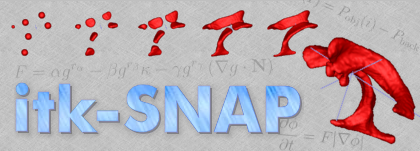
\includegraphics[width = 0.25\linewidth]{ITKSnapLogo}~~~~~
\includegraphics[width = 0.25\linewidth]{GlaLogo}~~~~~
\includegraphics[width = 0.1\linewidth]{GCEC}
\end{figure}
\newpage
\subsection*{Visualisation of .vtp/.vtk files}
For each frame submitted, there are now .vtp/.vtk files. These are the medial meshes of the submitted case with the applied labels and new biomechanical values that have been calculated. This data is best viewed in the free software, \href{https://www.paraview.org}{paraview}. 

The data now included are either specific to the points, to the cells, or are global data that are uniform over the whole field.

\subsection*{Data Summary}
~
\begin{tabular}{|c|c|l|}
	\hline
\textbf{Name}	& \textbf{Type} & \textbf{Description}   \\
	\hline
	\hline
	\multicolumn{3}{|c|}{\textbf{Root Anatomy}} \\
	\hline
STJ	& Scalar  & Marks the sinotubular junction with value 1 and 0 elsewhere.  \\
	\hline
VAJ	& Scalar &  Marks the ventriculo-aortic junction with value 1 and 0 elsewhere.  \\
	\hline 
IAS	&Scalar &Marks the interatrial septum with value 1 and 0 elsewhere. \\
	\hline
Label	& Scalar & ???\\
\hline
\hline
\multicolumn{3}{|c|}{\textbf{Point Root Properties}} \\
	\hline
Curv$\_$Gaussian	& Scalar& The gaussian curvature.\\
\hline
Curv$\_$Mean	& Scalar& The mean curvature.\\
	\hline
J$\_$Pt	& Scalar& The jacobian.\\
	\hline
I1$\_$Pt& Scalar & The principle strain. \\
	\hline
Motion	& Scalar& The motion of each point between the time frames.\\
	\hline
Total$\_$Motion	& Scalar& The cumulative motion. \\
	\hline
Radius	&Scalar & The distance from the wall centre to the wall edge.\\
\hline
Thickness	&Scalar & The wall thickness.\\
	\hline
Circ$\_$Strain$\_$Pt	& Scalar & The circumferential strain.\\
\hline
Long$\_$Strain$\_$Pt	& Scalar & The longitudinal strain.\\
	\hline
Circumferential$\_$Pt	& Vector &The circumferential vector. \\
	\hline
Longitudinal$\_$Pt	&Vector & The longitudinal vector.\\
	\hline
Normal$\_$Pt	&Vector & The normal vector.\\
	\hline
Displacement$\_$Wall & Vector & The displacement of the root wall, relative to the root centre. \\
	\hline
Displacement$\_$Root  &  Vector& The displacement of root, without the wall movement. \\
	\hline
Displacement$\_$Total & Vector & The displacement, with both the wall and root displacements. \\
\hline
\hline
\multicolumn{3}{|c|}{\textbf{Cell Root Properties}} \\
\hline
J$\_$Cell	& Scalar& The jacobian.\\
\hline
I1$\_$Cell& Scalar & The principle strain. \\
\hline
Circ$\_$Strain$\_$Cell & Scalar & The circumferential strain.\\
\hline
Long$\_$Strain$\_$Cell & Scalar & The longitudinal strain. \\
	\hline
Circumferential$\_$Cell	&  Vector  & The circumferential vector.\\
	\hline
Longitudinal$\_$Cell 	&  Vector & The longitudinal vector.\\
	\hline
Normal$\_$Cell 	&  Vector & The normal vector.\\
\hline
\hline
\multicolumn{3}{|c|}{\textbf{Global  Properties}} \\
\hline
Wall$\_$Area	&Scalar &The total wall area of the frame. \\
	\hline
	Wall$\_$Volume	&Scalar &The total wall volume of the frame. \\
	\hline
	Lumen$\_$Volume	&Scalar &The total lumen volume of the frame. \\	
	\hline
Valve$\_$Position	&Scalar & The valve is open when value is 1 or closed when value is 0.\\
	\hline
\end{tabular}
\\
\subsubsection*{Visualisation}
The exported .vtp files can be loaded in \href{https://www.paraview.org}{paraview}, where the frames can be cycled through. The movements of the root have been separated so that the wall movement, without the movement of the whole root, and the root movement, without the wall movement, can be viewed separately. The default has the movement fixed to the position of the reference frame. To view the movements, apply the `Warp By Vector' filter and chose the relevant displacement vector, with `Scalar Factor' set to 1. The vectors can be visualised with the filter `Glyphs'.

%\subsubsection*{CSV data files}
%Also included are two .csv files which contain average values and field values for each time frame. There is a raw data set, in which the time points are determined by the original frames submitted and the time between each. The second set has the the time standardised, so that different data sets can be more readily compared. It should be noted that, for the standardised time, it has been assumed that the cycle starts before when the valve opens and that the ratio of the valve being open to it being closed is 1:2.



\end{document}
